\documentclass[simplex.tex]{subfiles}
% NO NEED TO INPUT PREAMBLES HERE
% packages are inherited from simplex.tex; you can compile this on its own

\onlyinsubfile{
\title{NeuroData SIMPLEX Report: Subfile}
}

\begin{document}
\onlyinsubfile{
\maketitle
\thispagestyle{empty}

The following report documents the progress made by the labs of Randal~Burns and Joshua~T.~Vogelstein at Johns Hopkins University towards goals set by the DARPA SIMPLEX grant.

%%%% Table of Contents
\tableofcontents

%%%% Publications
\bibliographystyle{IEEEtran}
\begin{spacing}{0.5}
\section*{Publications, Presentations, and Talks}
\vspace{-20pt}
\nocite{*}
{\footnotesize	\bibliography{simplex}}
\end{spacing}
%%%% End Publications
}


\subsection{meda}

Matrix Exploratory Data Analysis (meda) is a package being developed to
allow for easy generation of modern summary statistics effective for
high-dimensional data analysis. 

\begin{itemize}
  \item Source code: \href{https://github.com/neurodata/meda}{https://github.com/neurodata/meda}
  \item Example output generated from Fisher's Iris data is here:
    \href{http://docs.neurodata.io/meda}{http://docs.neurodata.io/meda}
  \item The goal of the package:
    \href{https://github.com/neurodata/checklists/blob/master/matrix.md}{https://github.com/neurodata/checklists/blob/master/matrix.md}, the top five of which include summaries of data type, fraction of missing data values, generating heatmaps, and detecting outliers.
\end{itemize}

\subsubsection{Synaptome Statistics}

We have continued to examine the Kristina15 synaptome dataset and have
now added the Weiler Chessboard dataset to our explorations.  Using 
\verb+meda+, and other methods along the way, we have started to compare
the structure of these two datasets.  

\begin{figure}[h!]
\begin{cframed}
\centering
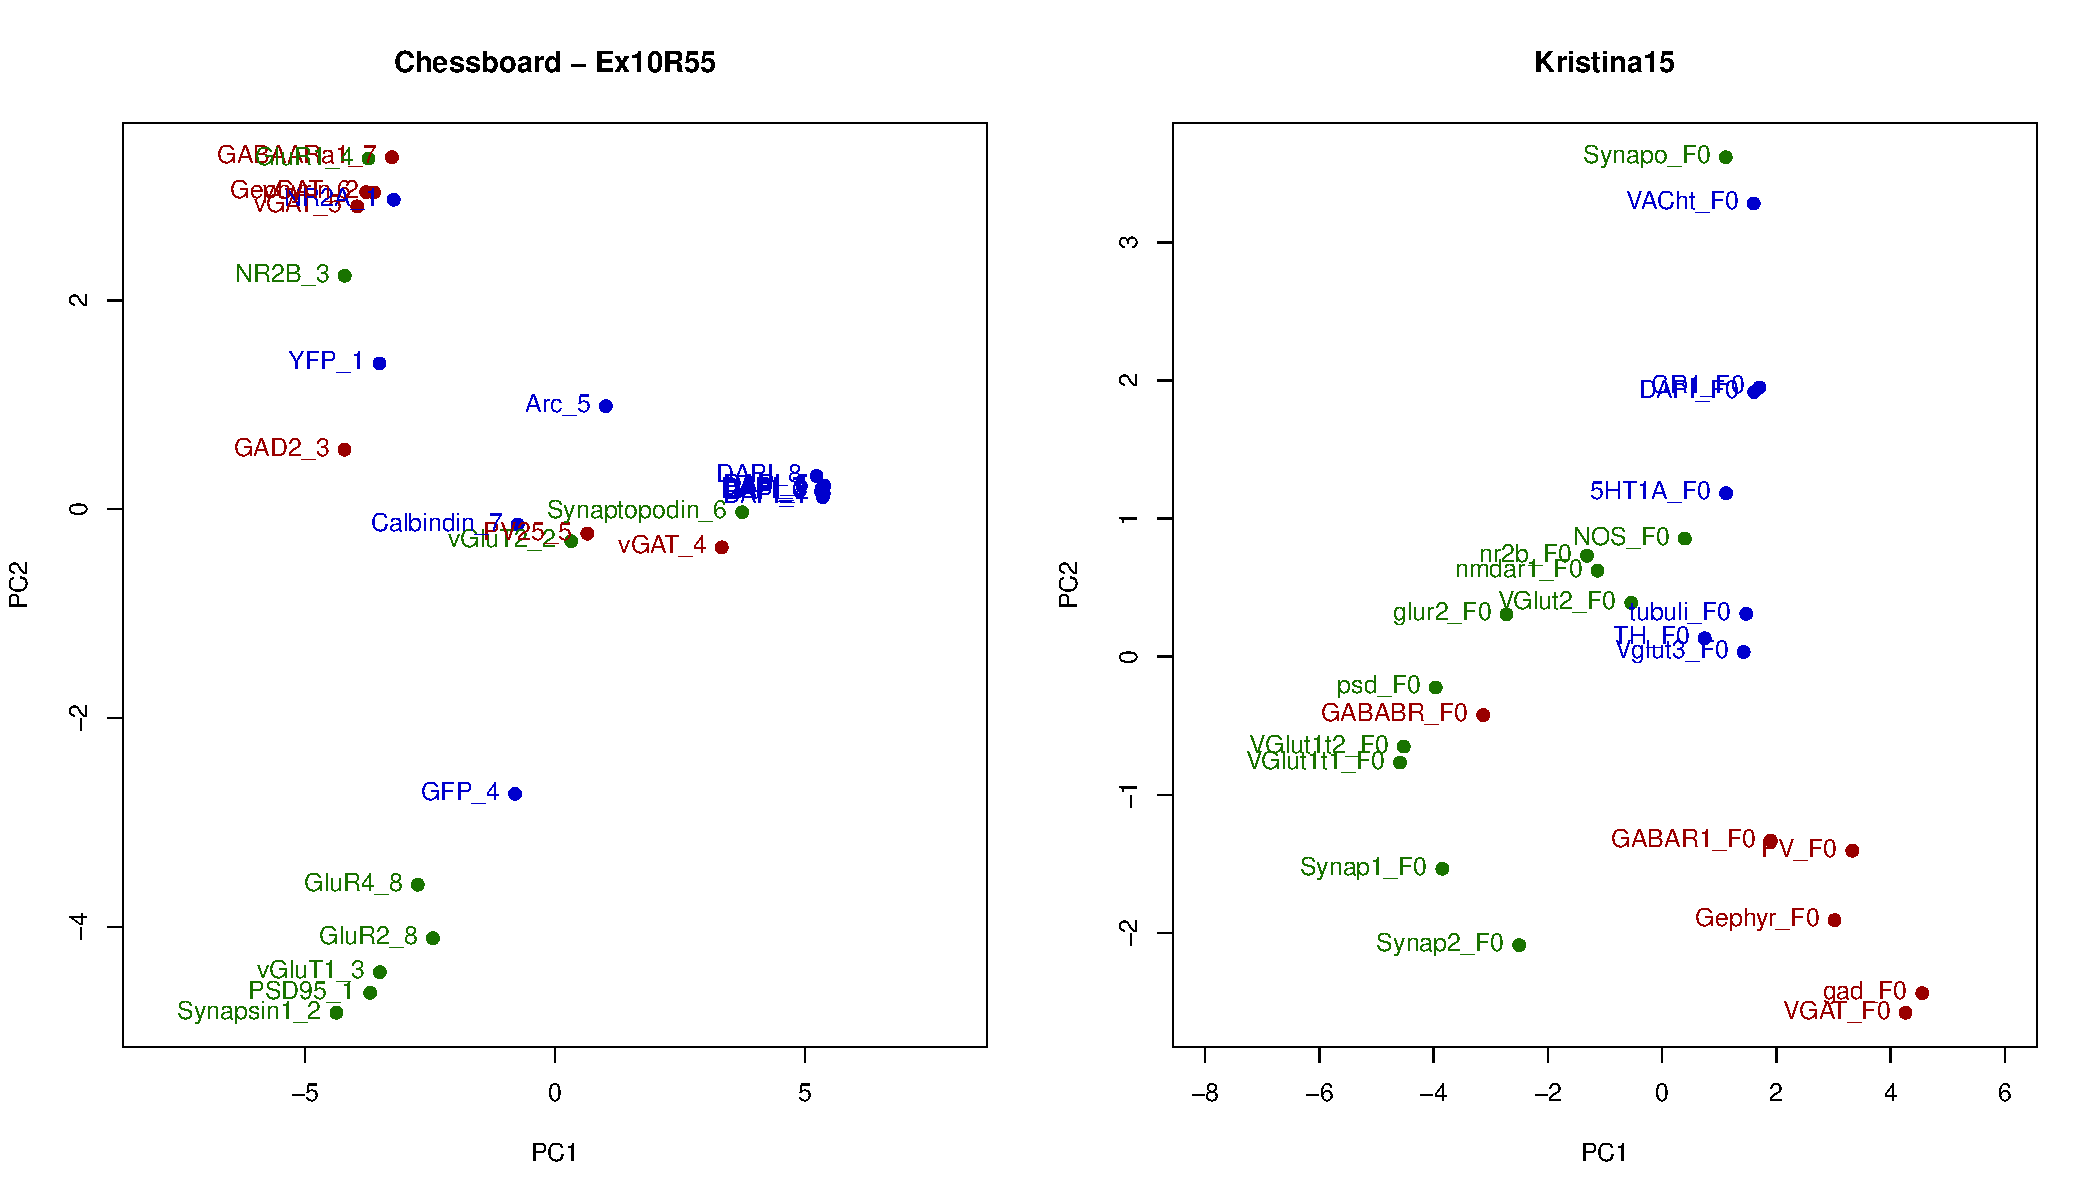
\includegraphics[width=\textwidth]{./figs/2dProjClaw.pdf}
\caption{
  Principal Component Analysis (PCA) has been run on the correlation
  matrices of both of these dataset respectively.  The first two
  principal components are plotted against each other.  The colors
  correspond to the type of marker, (``excitatory'' -- green,
  ``inhibitory'' -- red, ``other'' -- blue).  Notice that some markers are
  different between datasets, but there is a similar "claw" structure
  present. 
}
\label{fig:synClaw}
\end{cframed}
\end{figure}

\end{document}
